\chapter{Elephant Flow Monitoring} \label{chap:me} 

\section{Elephant flow detection algorithm}

\par Section \ref{sec:change_detection} presents several techniques for time series analysis and change detection, in which we explore the available 
techniques for modelling the data in a time series, calculating predictions from a time series' historical data (see equation \ref{eq:exp_smooth}), and 
finding change points in this data (see section \ref{sec:change_detection}). Using this mathematical baseline, we built an algorithm that monitors the changes
in the traffic characteristics of an interface of a switch. 

\par Algorithm \ref{alg:high_level} is a high level overview of the steps required to obtain the detection, and in the following sections, we introduce each step,
and provide some clarifications on the design decisions.

\begin{algorithm}[H]
    \caption{Elephant Detection Algorithm - High Level} \label{alg:high_level}
    \begin{algorithmic}[1]
        \Procedure {Elephant Flow Detection}{}
            \State Initialization
            \State Query controller
            \Loop
                \State Calculate prediction error
                \State Predict next values
                \State Detection
                \If {Detection}
                    \State Raise Alarm
                \EndIf
                \State wait 2 seconds
            \EndLoop
        \EndProcedure 
       \end{algorithmic}
\end{algorithm}

\subsection{Initialization}

\par In equation \ref{mat:port_stats}, $B_{XX}$ and $P_{XX}$ describe to the port statistics obtained from the controllers (see table \ref{tab:of_port_stats}), the 
byte (B\textsubscript{XX}) and packet (P\textsubscript{XX}) counters, respectively, and the indexes describe if the counters account for the transmitted or
received data in that port.

\begin{equation}
    \centering
    x_i = 
    \begin{bmatrix}
    B_{RX}\\
    P_{RX}\\
    B_{TX}\\
    P_{TX}\\
    \end{bmatrix}
    \label{mat:port_stats}
\end {equation}

The initialization step of the algorithm is a crucial step for obtaining correct results in the algorithm. Algorithm \ref{alg:init} defines the actual steps in this
algorithm, allowing the correct initialization of the model parameters, including the trend component, and to provide a baseline for the expected traffic on the
network. It is assumed that no traffic abnormalities exist during this stage, but a longer period for initialization can account for short bursts of higher traffic.

\begin{algorithm}[H]
    \caption{Elephant Detection Algorithm - Initialization} \label{alg:init}
    \begin{algorithmic}[1]
        \Procedure {Initialization}{}
            \State initialization period = 30s
            \While {t <= initialization period}
                \State x = Query controller
                \State initialization measures += x
            \EndWhile
            \State Linear Regression (initialization measures)
        \State \Return Linear regression coefficient
    \end{algorithmic}
\end{algorithm}

% XXX - justify the linear regression for de trending of the data

\subsection{Prediction and error calculation}

Time series analysis can generate forecasts for future values, assuming the temporal behaviour is maintained for future observations. A change detection mechanism
analyses the difference between the predicted value to the observation, by analysing the prediction error. In this section we present the prediction and error
calculation sections of the elephant flow detection algorithm.

\par For calculating forecasts, we have presented in section \ref{sec:forecasting} two possible methods for generating predictions. During the design phase of the 
algorithm, we selected the exponential smoothing technique, since this is a commonly used technique \cite{jasek_usage_2013, munz_traffic_2010} in the reviewed
literature, and provides a generally simple way to generate forecasts based in historical data. For readers convenience, the prediction equations are repeated 
here from section \ref{sec:math_form}, since they provide the mathematical baseline for the  development of prediction module of the algorithm. The equations are:

\begin{equation}
    \centering
        \begin {split}
            &\hat{x}_1 = x_0, \\
            &\hat{x}_t = \alpha x_{t} + (1-\alpha)x_{t-1}, t > 1.
        \end {split}
    \label{eq:exp_smooth_rep}
\end{equation}

\par With this method are able to predict the values that are expected in the following sample. In this step, the most important consideration is the adjustment of 
the forgetting factor, $\alpha (0 < \alpha < 1)$, that determines the impact of previous samples on the calculation of the prediction. The value of this factor must
be adjusted experimentally, by tuning the value according to the desired output.

\par For calculating the prediction error $\epsilon_t$, we have analysed two possibilities. The first, obtained with

\begin{equation}
    \centering
    \label{eq:division}
    \epsilon_t = (x_i(t)/\hat{x}_i(t))^2,
\end{equation}

\par provides the output present in figure \ref{fig:error_plot_division}, and while it clearly indicates the deviations created by the elephant flows, it 
does not provide insight to the level of change caused by larger payloads in the flows.

\begin{figure}[H]
    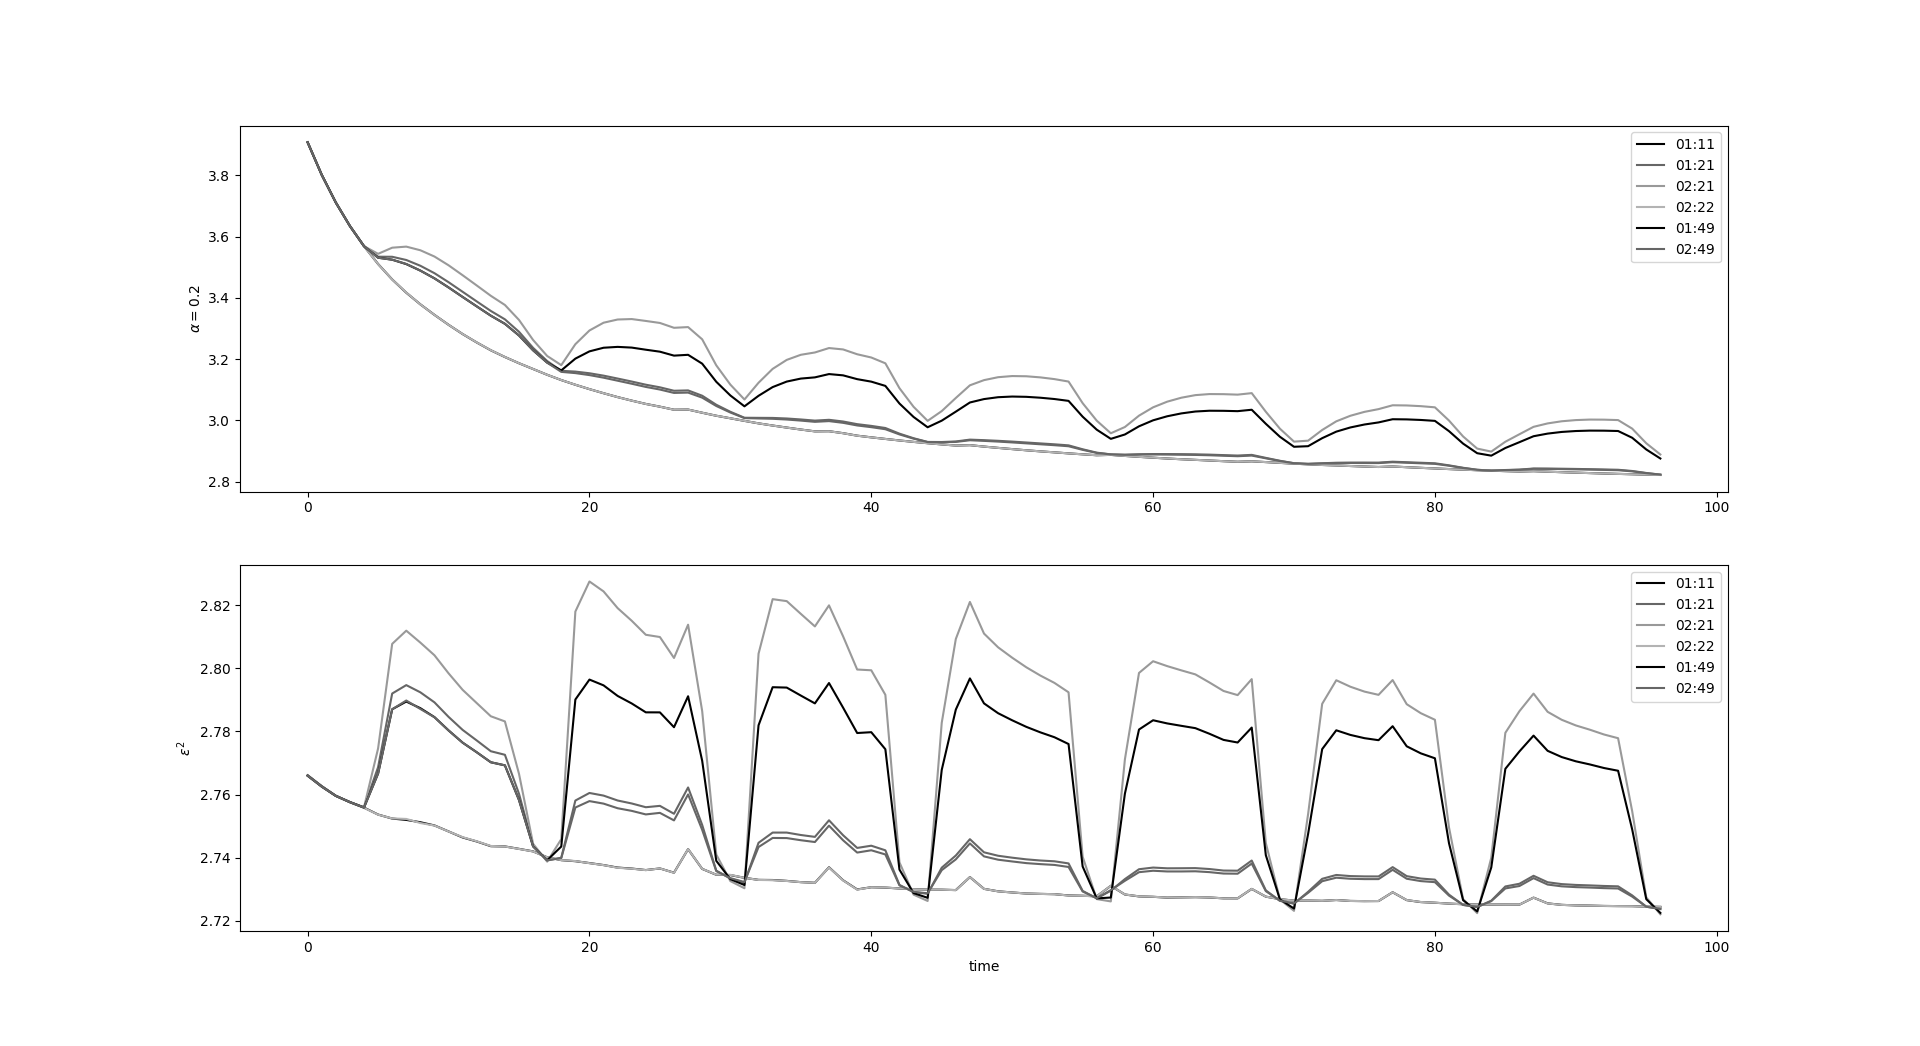
\includegraphics[width=1.2\textwidth]{meter_eleph/error_plot_division}
    \caption{Error calculation, with two different values for $\alpha$, obtained with equation \ref{eq:division}}
    \label{fig:error_plot_division}
\end{figure}

\par The alternate approach devised was to consider the squared prediction errors, as shown in equation \ref{eq:sse_rep}.

\begin {equation} 
    \label{eq:sse_rep}
    \epsilon_t^2 = (x_t-\hat{x}_{t})^2 
\end {equation}

This method allows to obtain the prediction error, while increasing the impact of larger changes to the flow data size, and minimizing smaller changes. In figure
\ref{fig:error_plot_sse} we can visualise the output of this method, which displays the traffic behaviour in the ports of a switch, and the impact of larger payloads
of data is visible, as shown by the increasing level of $\epsilon_t$.

\begin{figure}[H]
    \label{fig:error_sse}
    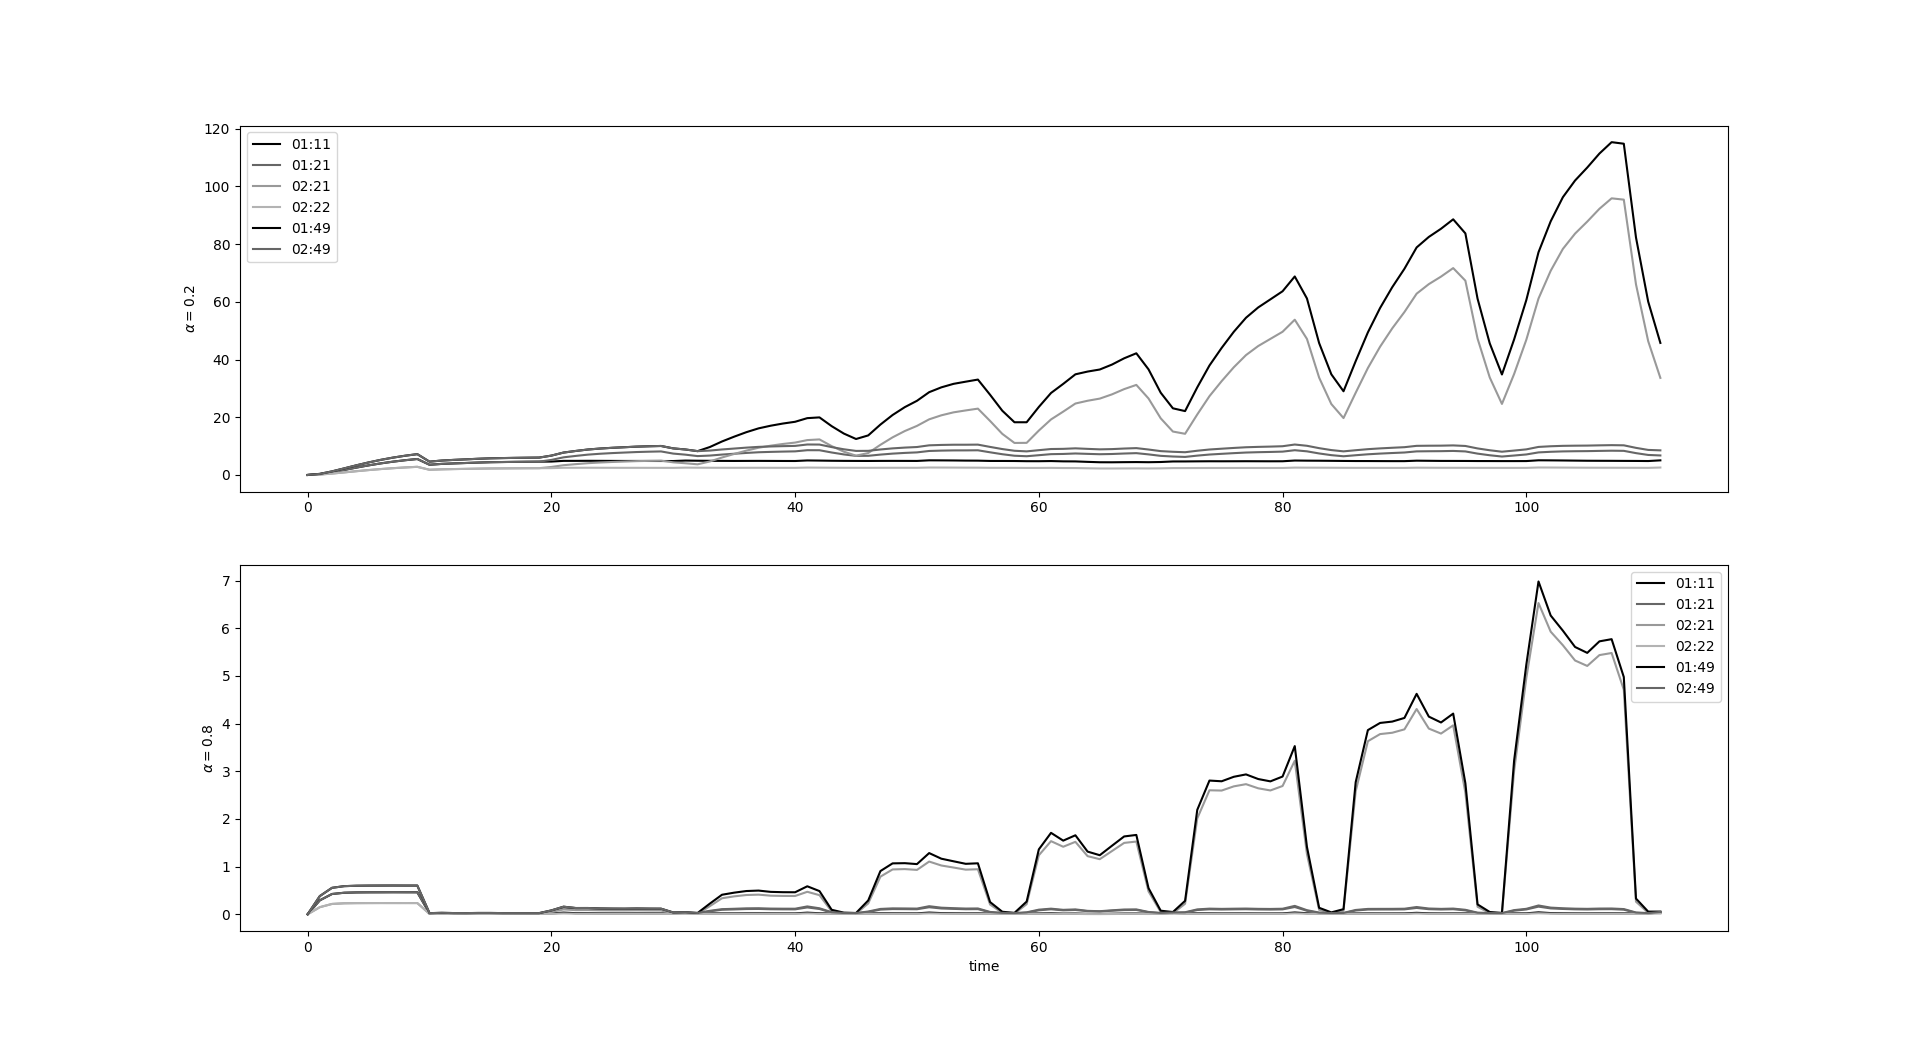
\includegraphics[width=1.2\textwidth]{meter_eleph/error_plot_sse}
    \caption{$\epsilon^2$ calculation using the method present in \ref{eq:sse_rep}}
    \label{fig:error_plot_sse}
\end{figure}

\par In figure \ref{fig:error_plot_division} and \ref{fig:error_plot_sse} , we test the error prediction behaviour for two different values of the $\alpha$ parameter
of the prediction equations, to see the impact that the previous observations have on the error behaviour. We consider the output of the bottom plot of 
\ref{fig:error_plot_sse} as the desired one, where we assume $\alpha = 0.8$ since it clearly indicates the start and end times of the variation, which in contrast 
to the upper plot in this figure, where the value $\alpha = 0.2$ is used, does not present a rising trend. Due to this result, we propose higher ($\alpha \rightarrow 
1$) values for the smoothing factor for posterior results, more specifically $\alpha = 0.8$.

\subsection{Detection}

The detection component of the algorithm provides the logic for finding the timestamps where a port's traffic behaviour changes. For this component we consider two
possible techniques: the first, which simply compares the output of the error calculation to a certain threshold; and a second, using the CUSUM algorithm (see 
section \ref{sec:change_detection}).

\par The first analysed detection method is defined as

\begin{equation*}
    \centering
    \label{eq:detection_method}
    \epsilon^2 \geq \delta,
\end{equation*}

\par and this method provides advantages mainly due to the simplicity of the technique, however previous knowledge of the change is required to determine a
possible threshold $\delta$.

\par The second analysed method is the CUSUM algorithm. This method is used for monitoring parameters of a sample, by monitoring deviations of the observations
according to a certain target value. Typical implementations of this algorithm are based in an offline approach, calculating the alarm times with knowledge of the 
entire data set. Since our method is expected to run in an online approach, the adaptation of this algorithm for an online form is based in the application of a 
sliding window of observations.

\par The offline method allows us, however, to obtain a baseline for the online detection algorithm. We have collected the error prediction output, and applied the
algorithm to a generated data set. Performing this step baselines the expected number of alarms that are raised in a certain testing conditions, so that application
of the online algorithm may provide the closest approximation to the optimal offline version. The chosen CUSUM algorithm implementation used was from 
\url{https://github.com/demotu/BMC}, and  figure \ref{fig:offline_cusum} shows the alarms raised. Furthermore, this implementation also provides us with the
timestamps corresponding to the start and end of the detected changes. This algorithm calculates the CUSUM of a set of data, and expects two inputs:
a threshold parameter, which defines the amplitude threshold for the change in data; and the drift parameter tunes the algorithm to allow faster detection (larger 
drift), or less false alarms (smaller drift). 

\begin{figure} [H]
    \centering
    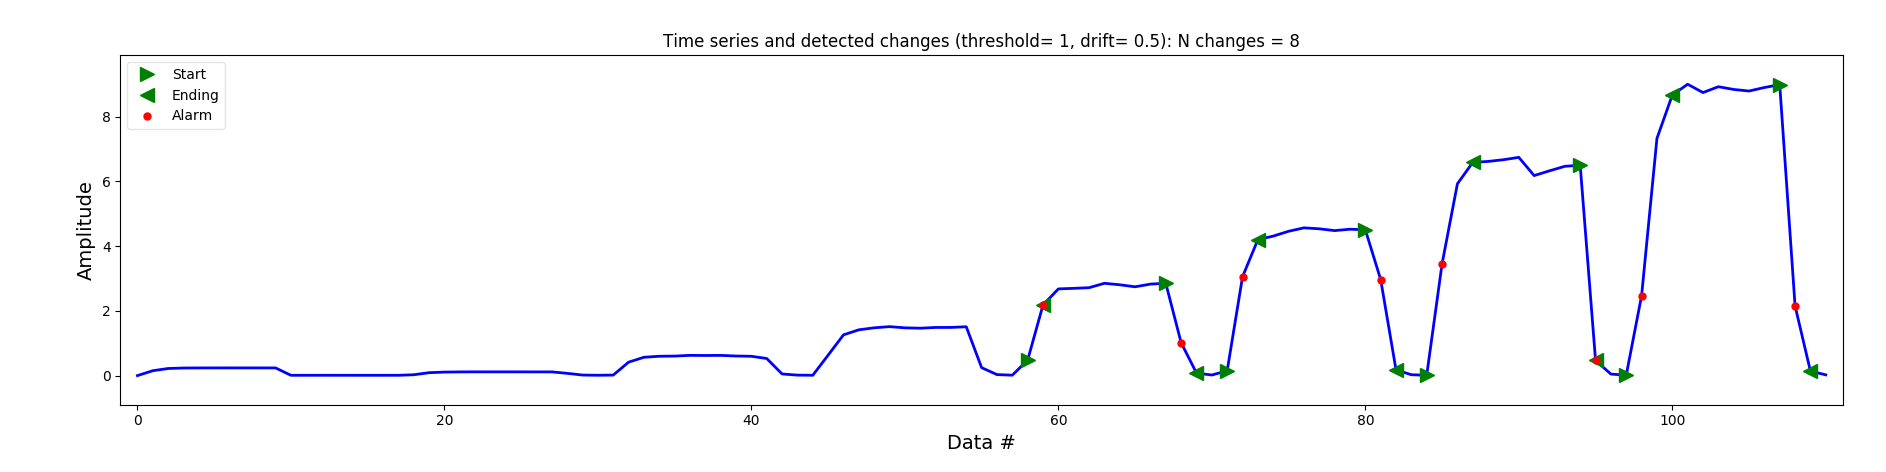
\includegraphics[width=1\textwidth]{meter_eleph/offline_cusum_output}
    \caption {Offline CUSUM output}
    \label{fig:offline_cusum}
\end{figure} 

\par The adaptation of the CUSUM algorithm for utilization as an online technique is based on a sliding window that is updated with every new sample. Applying this
method has the advantages of using the CUSUM algorithm without needing extensive changes, while also reducing the amount of memory needed to apply this method. 
Choosing the window size is a central point to a successful implementation of the change detection mechanism, that is explored further in section 
\ref{sec:change_results}. 

\section {Testing}

The design of a testing environment for testing of the change detection algorithm, must allow for the accurate simulation of the traffic conditions on real DCNs,
and should provide the flexibility to understand and change the underlying topologies. This indicates a strong motivation for deploying a testing environment in a
virtualised environment, using tools like \textit{mininet}, which provides a miniature network that can be changed as needed. This testing suite provides a strong
alternative to deploying these changes in hardware.

\par Despite the changes implemented to Basebox, utilizing these controllers in combination with the virtualised environment poses a challenge, related 
to the implementation of the OpenFlow protocol in the hardware and software switches. Hardware switches that were used for the implementation of
the OSS have a modified version of the OpenFlow tables structure, OF-DPA (see section \ref{sec:ofdpa}), and the libraries that make up the 
controller are designed around this. To utilize the controllers, changes to Open vSwitch or other alternatives steps would be required in order to use the
environment, which was decided out-of-scope for this thesis.

\par To solve this issue we adopt a different controller for interaction with the virtual environment. In addition, researching the traffic engineering modules in
other controllers provides ideas that can later be adopted in Basebox. The chosen controller was Floodlight (see section \ref{chap:flood}), since it exposes a simple
REST API for obtaining statistics, setting table rules, and is continuously maintained providing an optimal test bed.

\par These elements compose the testing environment that seen in \ref{fig:test_setup}. To ease the installation of the utilized applications, 
we based these applications on VMs and containers, and the installation files can be found on github \footnote{\url{https://github.com/rubensfig/thesisdoc.git}}.

\begin{figure} [H]
    \centering
    \includegraphics[width=0.6\textwidth]{meter_eleph/testing_setup}
    \caption {The high level overview of the testing setup}
    \label{fig:test_setup}
\end{figure} 

\par Figure \ref{fig:test_setup} describes the testing setup designed for testing. This setup provides a close approximation to setups used
to the Top-of-Rack switches connected to the servers on the edge layers (see figure \ref{fig:fattree}) of data centers, while keeping the resource consumption of
the virtualised network and controller to a minimum. In the diagram, the hosts are shown using the H\textsubscript{X} notation, ranging from 1 to 4, and the switches
use the S\textsubscript{X} notation. Information about the hosts, like the IP and MAC addresses can also be seen, and the port numbers used are also displayed.

Mininet provides an API to interact with a virtual network and setup tests in a predictable manner. We utilize this API to develop a script that creates the network
topology. For traffic generation, however, we require another tool that provides specific functionalities like control of the inter-packet interval and the packets 
payload size. The tool \textit{hping} is a common tool used for packet generation and port mapping, and its simplicity allows to quickly deploy different tests
against the designed setups. In picture \ref{fig:hping_setup} the command line interface of the tool is presented and the arguments to build the tests are presented.

\begin{figure}[H]
    \centering
    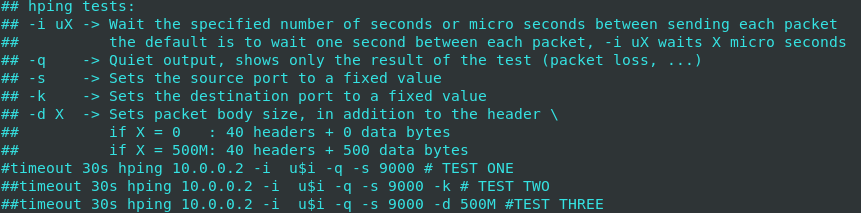
\includegraphics[width=0.9\textwidth]{meter_eleph/testing_link}
    \caption{hping tool tests and command line arguments}
    \label{fig:hping_setup}
\end{figure}

\par We consider a test scenario, where every host is communicating with each other, simulating background traffic. This has the purpose of simulating low traffic 
intensities in the network, and verify the behaviour of the designed algorithm in an approximation to real conditions. In this test scenario, we initialize the 
network with the background traffic for a specified amount of time, where we assume no abnormal traffic conditions. After this initialization period, we generate
traffic between the hosts H\_4 and H\_2 during a period of 30 seconds, increasing the payload of the packets each time.

% XXX - Find a citation for this, cant find it anywhere
\par The utilization of Open vSwitch has, however some limitations that should be address when the tests are being designed. Figure \ref{fig:ovs_packet_loss} shows
the increase of the packet loss as the number of flows in OVS increases. This limitation implies that in order for the tests to run successfully, there needs to be
a care in the amount of flows that are generated.

\begin{figure} [H]
    \centering
    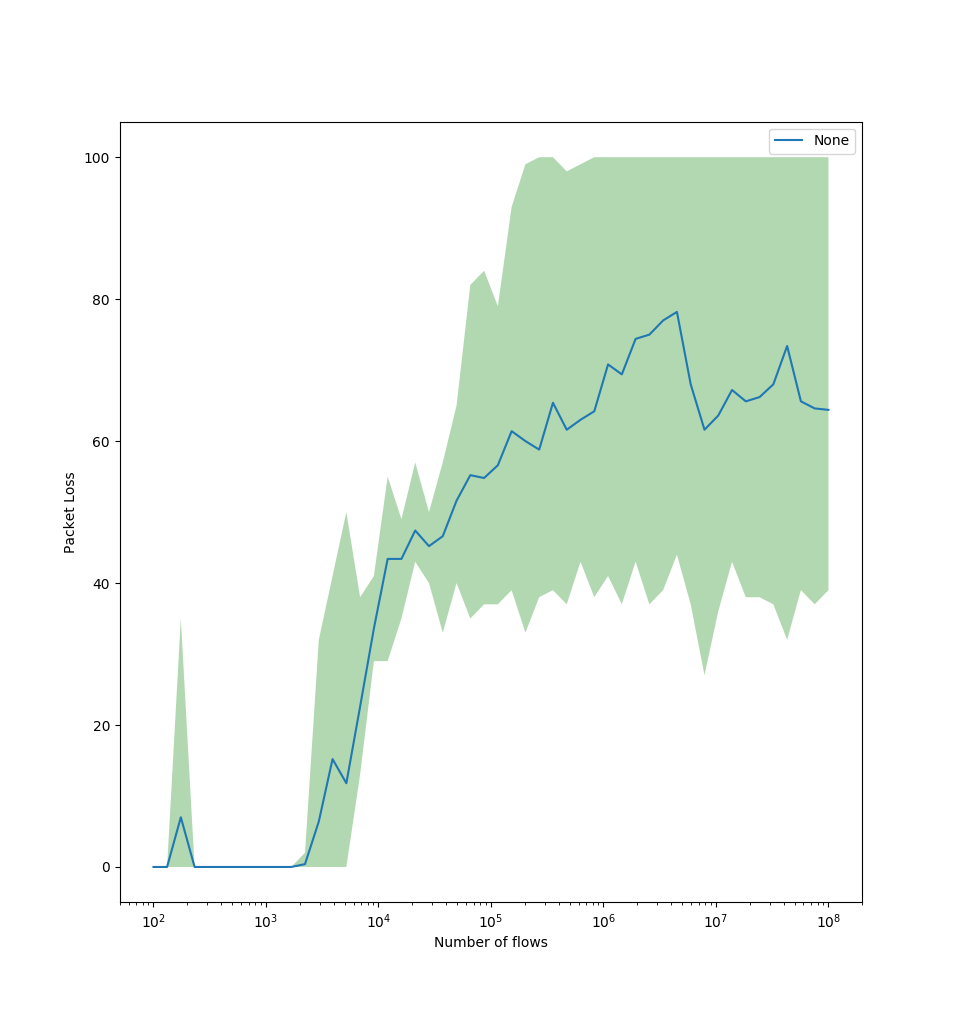
\includegraphics[width=0.6\textwidth]{meter_eleph/ovs_packet_loss}
    \caption {OVS measured packet loss}
    \label{fig:ovs_packet_loss}
\end{figure} 

\section {Results and Evaluation} \label{sec:change_results}

\par We analyse the measurements of the initial received bytes in the different ports of the switch. Figures \ref{fig:init_plot} and \ref{fig:init_plot_pkts} provide
an insight on the initial traffic characteristics of each port, and we observe that the ports providing the connection between the two switches report a higher
utilization in number of bytes and packets received. This figure also gives an insight on the present trend in the data, that in order to improve the next
values' prediction and error calculation, these trends should be removed.

% Display initial graph of Received Bytes
\begin{figure}[H]
    \centering
    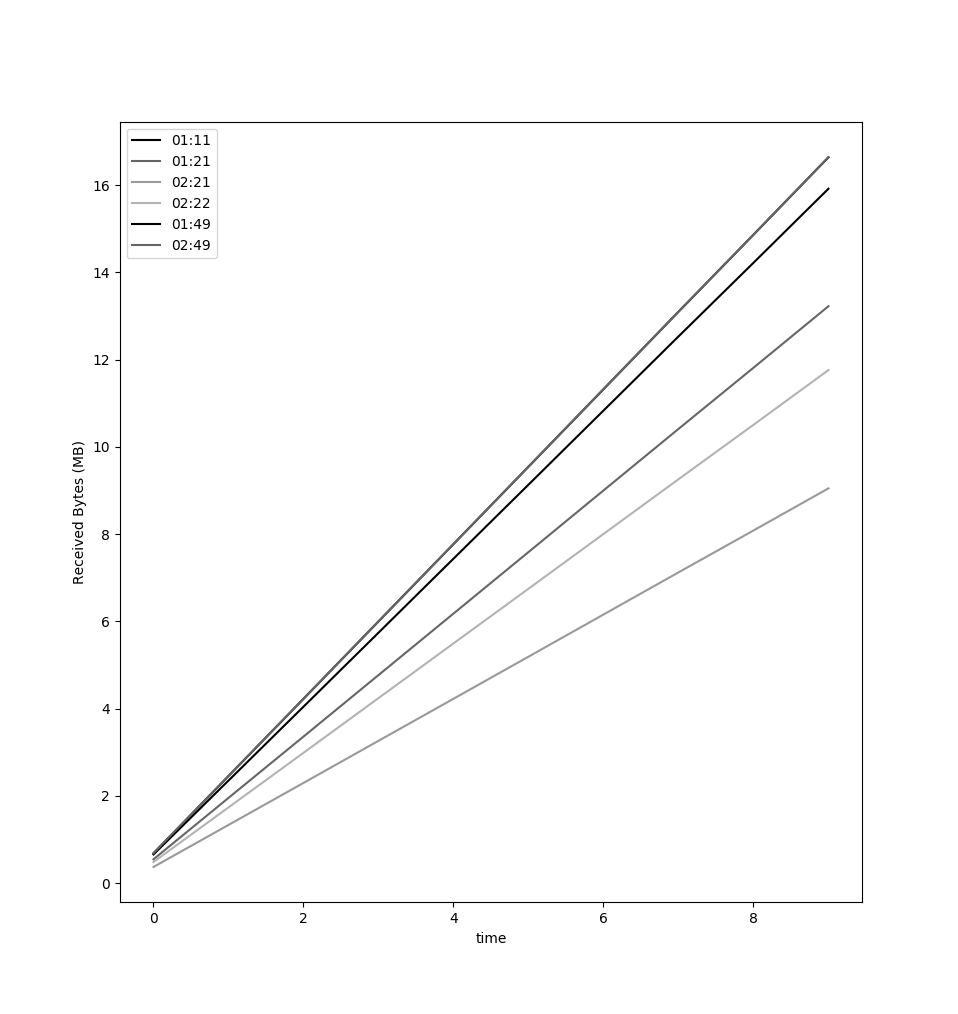
\includegraphics[width=0.6\textwidth]{meter_eleph/init_period_lin}
    \caption {Plotting the initial measurements of B\textsubscript{RX}}
    \label{fig:init_plot}
\end{figure} 

\begin{figure}[H]
    \centering
    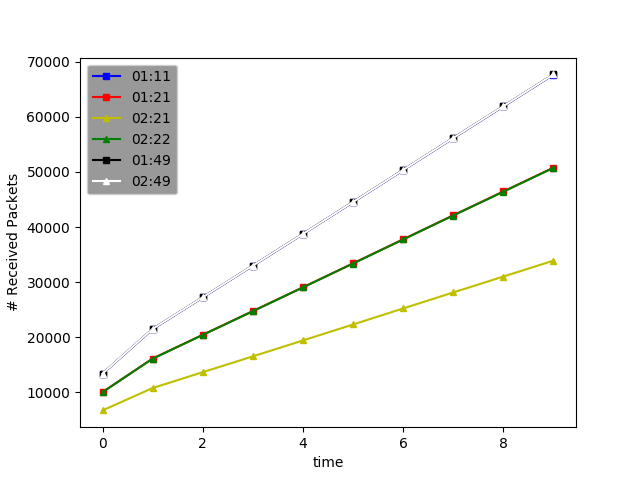
\includegraphics[width=0.6\textwidth]{meter_eleph/init_period_packets}
    \caption {Plotting the initial measurements of P\textsubscript{RX}}
    \label{fig:init_plot_pkts}
\end{figure} 

\par In the initial detection strategy, the error detection is based in comparing the calculated prediction error to a certain threshold. Choosing this threshold 
requires previous knowledge of the magnitude of the change, and figure \ref{fig:detect_dumb} represents the output of the prediction error calculation using this
method. We assume a value of $\delta > 2$ for this detection threshold, to show that the detection threshold may be tuned depending on the use case.

\par In figure \ref{fig:detect_dumb} we plot the prediction error calculated for every port on the switch, including the inter-switch connection. Since the developed
algorithm monitors the changes in traffic characteristics on the switch ports connected to a host, applying the change detection to the inter-switch connection
does not provide any useful information, as such, we do not apply the algorithms to these ports.
%in figure \ref{fig:detect_dumb}.

\begin{figure}[H]
    \centering
    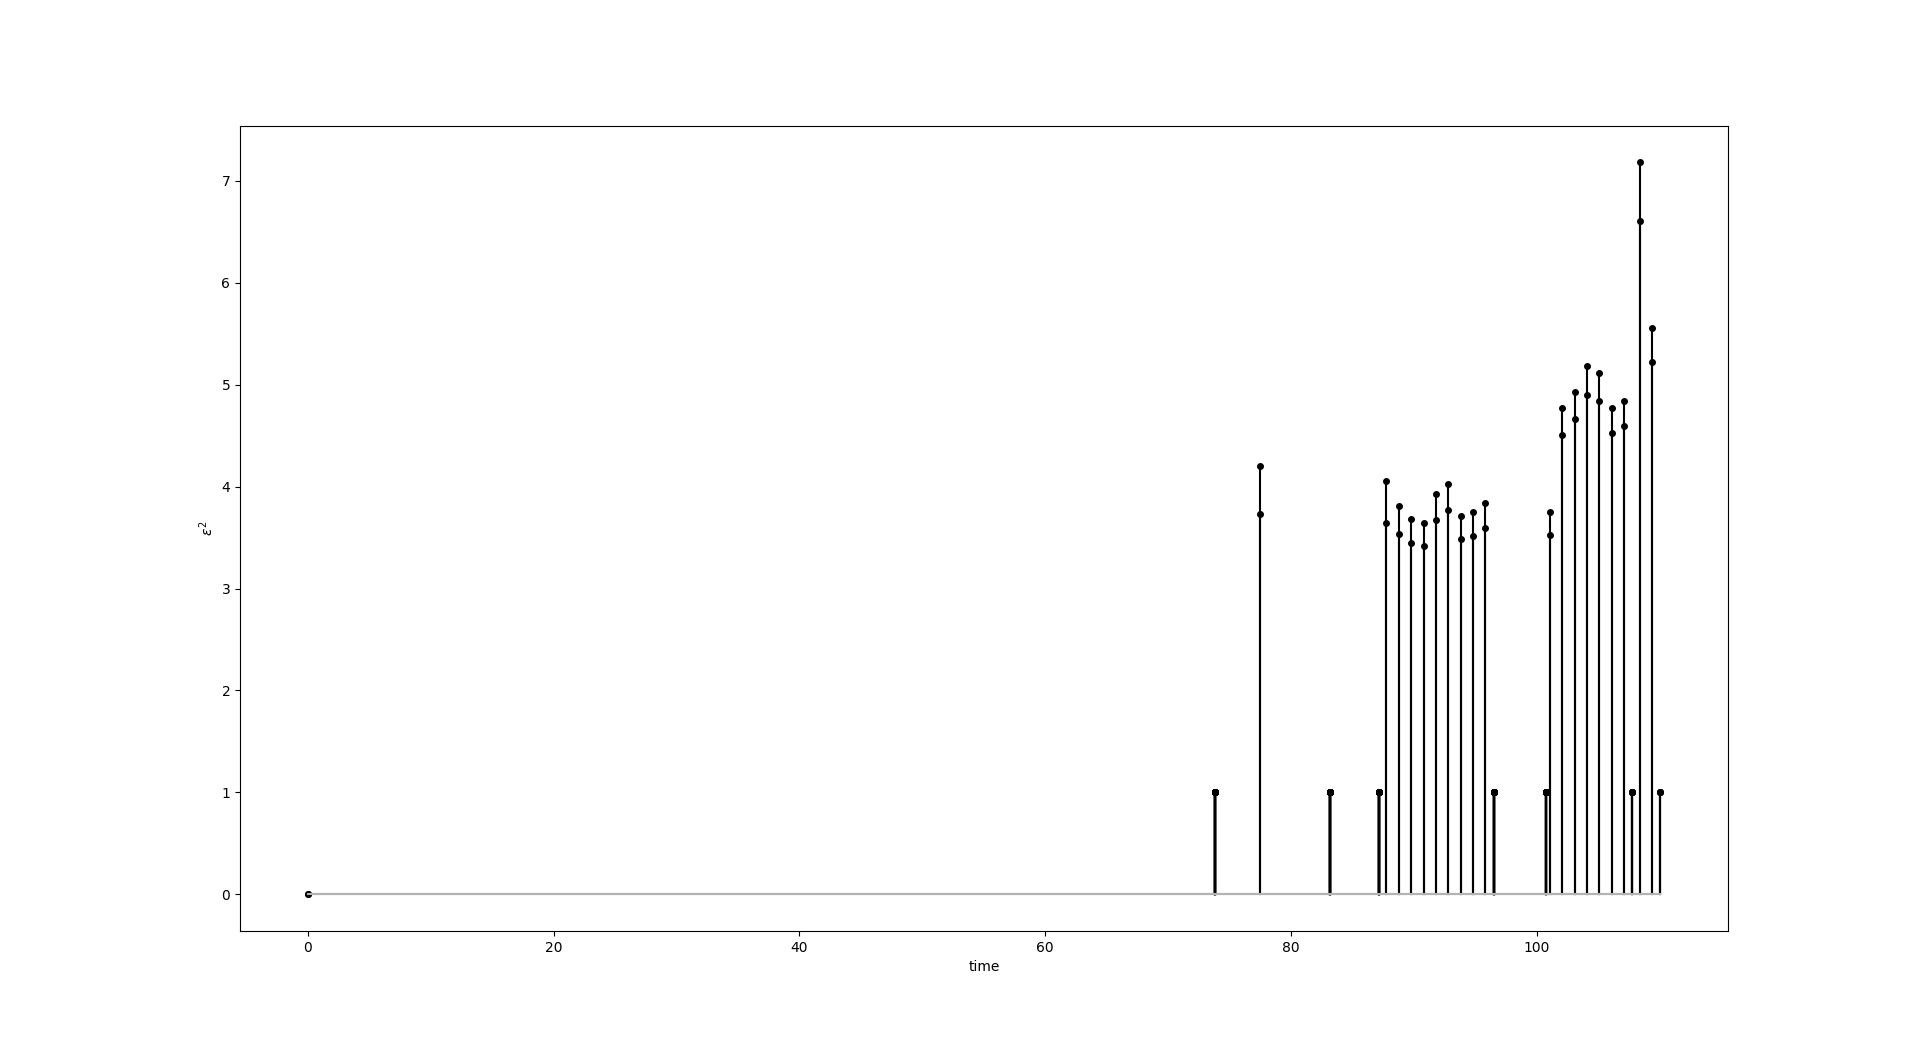
\includegraphics[width=.8\textwidth]{meter_eleph/detect_dumb}
    \caption {Simple detection}
    \label{fig:detect_dumb}
\end{figure} 

\par Figure \ref{fig:color_plot} displays the error detection using the CUSUM algorithm, and the timestamps of alarms raised for the switch port connected to
host H\textsubscript{4}. From this result, we conclude that with this algorithm we can accurately detect the changes in traffic per port. The greatest difference to
the previous mechanism is the reduction in the number of alarms, since this algorithm does the detection across a sliding window of observations, and the alarms are
only raised when the traffic characteristics change. Regardless, the same changes in port traffic are detected.

\begin{figure}[H]
    \centering
    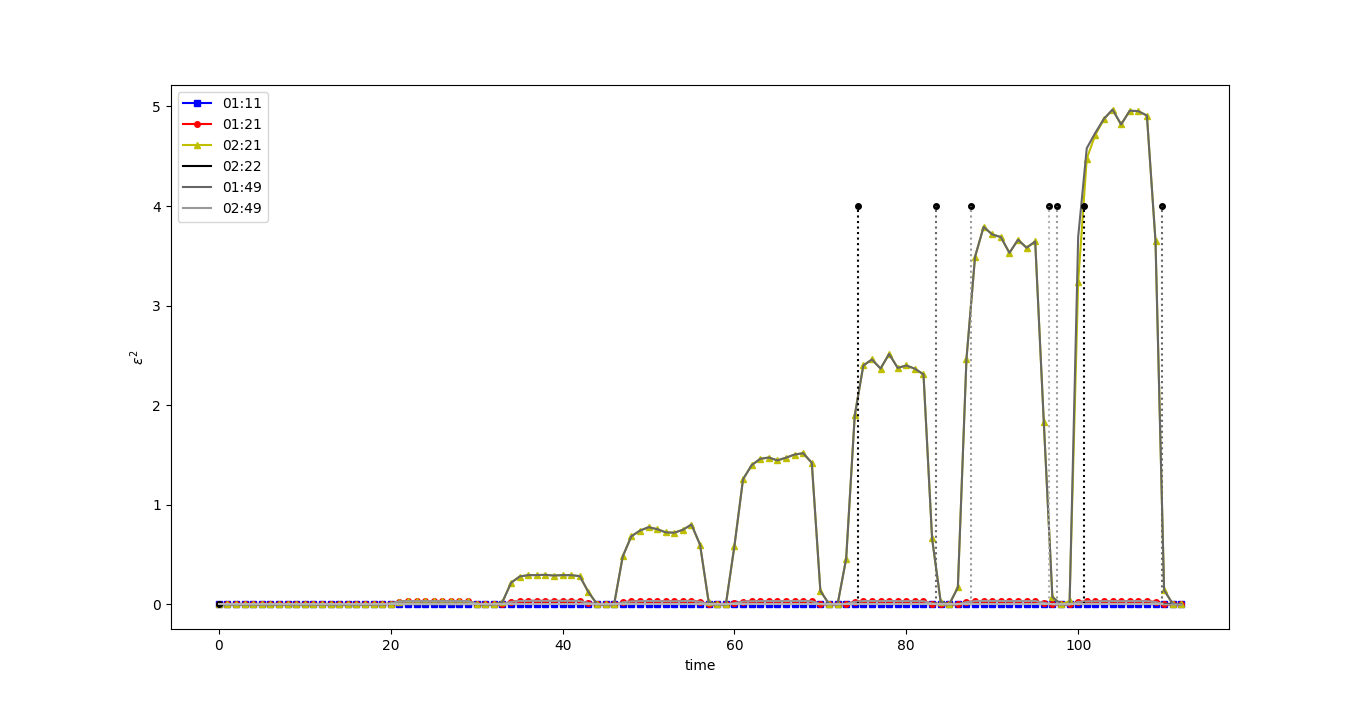
\includegraphics[width=.8\textwidth]{meter_eleph/detection_results_plotted}
    \caption{CUSUM Detection results}
    \label{fig:color_plot}
\end{figure}

\par Analysing the output of the algorithm after the tests finish indicates the corresponding timestamps of the alarms. Blindly applying the sliding window technique
in the algorithm will result in repeated alarms across the window, and as we vary the length of the window, the algorithm may raise notifications even if the change
has taken place at some time in the past. A simple enhancement to the proposed algorithm is to consider only the first occurrence of the alarms. Figure
\ref{fig:errors_comparaison} shows the result of plotting the number of alarms against the changing size of the window, the upper figure considering only the
timestamps of the first occurrence of the alarm, on the contrary of the lower figure.

\par This proposed approach also allows the comparison between the offline and the online approach to change detection. In figure \ref{fig:offline_cusum}, the 
offline output can be analysed for the number of expected alarms on this testing scenario. Comparing this result to the enhanced version in figure 
\ref{fig:errors_comparaison}, we conclude that the number of errors are similar to the offline version, which means that we can accurately detect every change in
the test scenario with the online algorithm.

\begin{figure}[H]
    \centering
    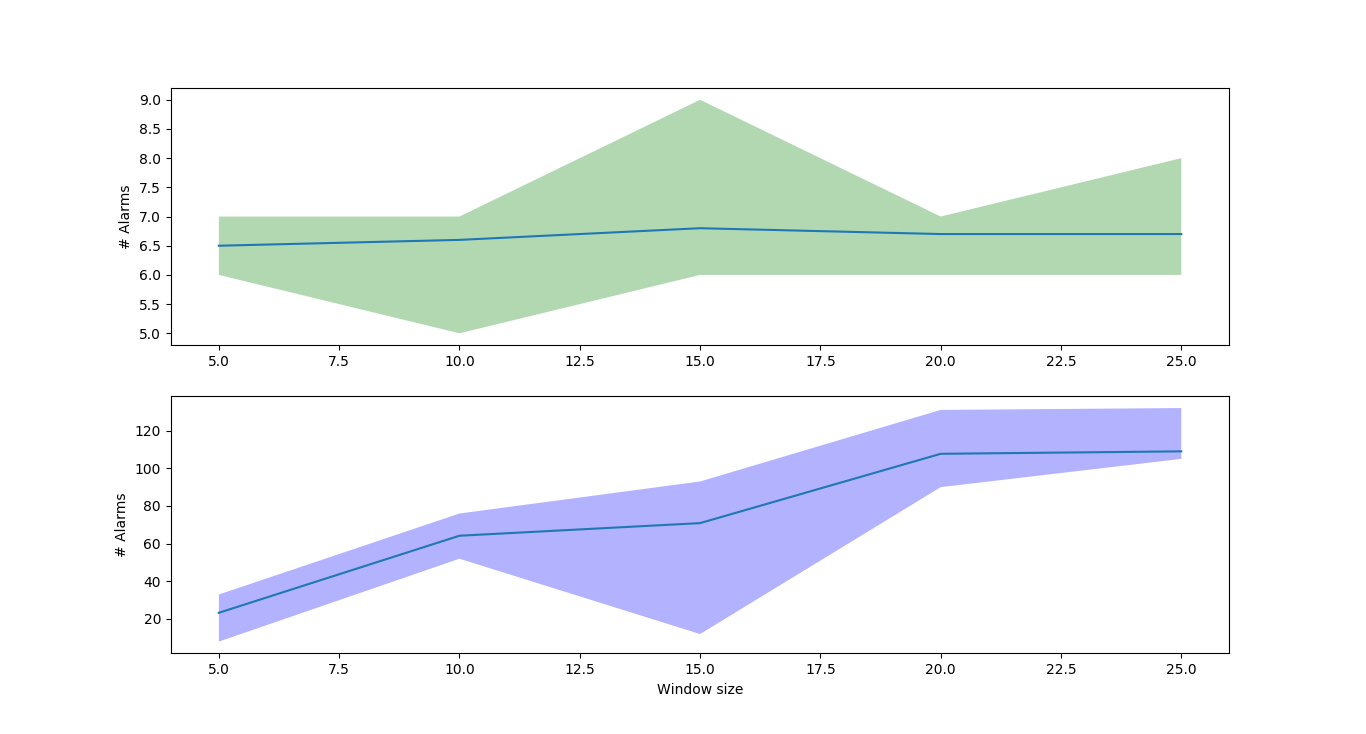
\includegraphics[width=.7\textwidth]{meter_eleph/evaluation_error}
    \caption {Comparison of the alarm count between enhanced and non enhanced version}
    \label{fig:errors_comparaison}
\end{figure} 

\par Continuing the analysis of the impact caused by the variation of the window size, the analysis of a single elephant flow (as shown in figure 
\ref{fig:single_elephant}) allows us to evaluate the performance of the algorithm, with the methods mentioned in section \ref{sec:performance_evaluation}. Obtaining
a baseline for the amount of raised alarms and detection timestamps was done by applying the offline CUSUM algorithm to this test case.

\begin{figure}[H]
    \centering
    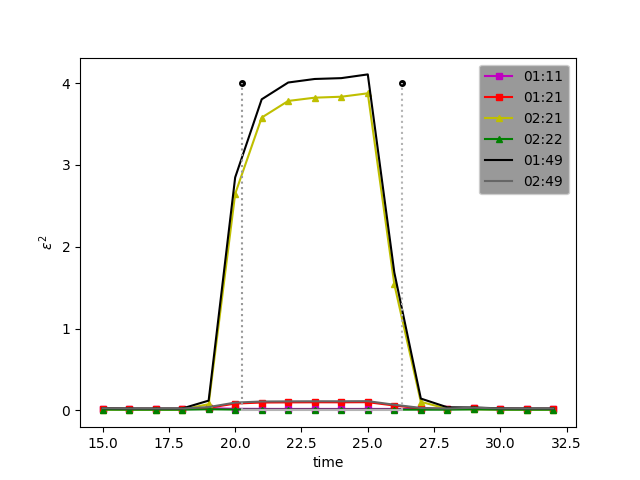
\includegraphics[width=.7\textwidth]{meter_eleph/single_elephant_flow}
    \caption{Single elephant flow}
    \label{fig:single_elephant}
\end{figure} 

\par The analysis of the error detection time will provide us with the performance of this change detection algorithm. By establishing the baseline detection times
obtained from the CUSUM algorithm, using the same threshold and drift parameters in the online and offline case, we can determine the difference between these
baseline values and the values obtained online. Figure \ref{fig:time_error} shows the result of this analysis, and the variation caused to the time to detection
from the varying window size. To generate this result, we have performed 30 different measures for each window size, and compare the time of detection to the baseline
value. 

\begin{figure}[H]
    \centering
    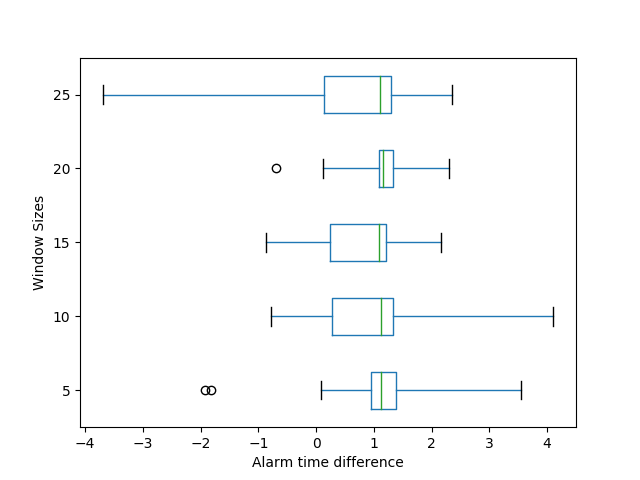
\includegraphics[width=.8\textwidth]{meter_eleph/time_error}
    \caption{Analysis of the time to detect the change}
    \label{fig:time_error}
\end{figure} 

\par Analysing the single elephant flow, and the output of the online detection algorithm also allows us to compare the baseline amount of alarms. This will give 
us an insight to the amount of false alarms generated, and the relationship of these with the window size. Figure \ref{fig:false_alarms} shows us the obtained
statistics of the number of alarms, which confirms a worse accuracy for the number of alarms with the smaller windows.

\begin{figure}[H]
    \centering
    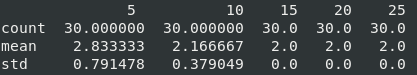
\includegraphics[width=.8\textwidth]{meter_eleph/false_alarms}
    \caption{Smaller window statistics}
    \label{fig:false_alarms}
\end{figure} 

\par In spite of the expected result of quicker detection for smaller windows \cite{choudhary_runtime-efficacy_2017}, figure \ref{fig:time_error} does not present 
much variation in the detection time, but the amount of false alarms raised by the smaller windows suggest a better performance of the algorithm using larger 
window sizes.

\par Finally, an interesting consequence of applying a change detection method applied to the statistics on the ports on the switch, is the independence of the 
protocol, allowing us to understand traffic changes on the ports regardless if the transport protocol is TCP or UDP.
% XXX image ??
